\section{Introduction}

\subsection{Overview of High-Frequency Trading and Reinforcement Learning}
High-frequency trading (HFT) represents one of the most technologically demanding domains within quantitative finance,
characterized by its need for ultra-low latency, massive volumes of data, and the ability to adapt dynamically to rapidly changing market conditions.
Reinforcement learning (RL) has emerged as a promising approach for developing trading strategies,
offering the ability to learn optimal policies directly from market interactions without requiring explicit rules or models.
However, applying RL to HFT is fraught with challenges, particularly when scaling training and inference to meet the performance
requirements of live trading environments.

Traditional RL frameworks often rely on centralized architectures, where a single learner aggregates experiences from multiple actors to update a shared policy.
While effective in general-purpose applications, such approaches can become bottlenecks in HFT contexts,
where the scale and complexity of trading environments demand distributed efficiency and continuous adaptability.
Moreover, typical RL systems treat environments as isolated entities for each agent or strategy,
leading to significant computational redundancies when simulating complex environments like the limit order book (LOB).

\subsection{Motivation and Contributions}

This thesis proposes a novel parallel, agent-based RL framework designed specifically for the HFT domain.
The framework leverages Ray RLlib to parallelize environments and adopts a structure inspired by the actor-learner model introduced in the
IMPALA (Importance Weighted Actor-Learner Architecture) algorithm.
However, it extends this paradigm by allowing multiple learners to share parallelized environments, each corresponding to a unique agent definition,
and enabling workers from different learners to share the same LOB environment.
This design reduces computational overhead by reusing core environment components, such as order aggregation, order book initialization,
and transaction processing, across multiple agents, and therefore reduces memory consumption and processing latency.

The primary contribution of the thesis is to provide a scalable, efficient, and adaptable framework for training RL agents in HFT applications, with the following key features:

\begin{itemize}
    \item A parallel agent-based framework: A pragmatic implementation of a system architecture that enables efficient and decoupled training of multiple RL agents
    by leveraging distributed computing resources.

    \item Shared limit order book environments: An innovative mechanism for reducing redundant computations by allowing multiple workers,
    assigned to different learners, to interact with shared reusable LOB environment.

    \item Continuous train-and-deploy pipeline: The framework aims to support dynamic training and deployment of multiple strategies,
    where real-time updates to agent policies can be made without interrupting the trading process.
\end{itemize}

The framework must scale effectively with the number of agents, learners, and environments, maintaining consistent performance as workload increases.
Performance metrics will include speedup and multicore efficiency, processing latency per action and end-to-end latency from state observation to order sending.
The framework will be evaluated for its ability to support diverse trading strategies
and market conditions through strategy-agnostic performance and modular design,
enabling the reconfiguration of agent definitions and environments with minimal overhead.
Additionally, the feasibility of deployment in live trading systems will be assessed through backtesting with simulated market data,
where agents will be evaluated based on their loss and reward scores, and therefore assess their ability to adapt to changing market conditions.

The final thesis structure will first review relevant literature and novel approaches towards distributed agents
in reinforcement learning and intersections with high-frequency trading, specifically parallel agent-based frameworks.
An adequate search string will be fabricated, and a systematic review will be conducted to identify the most relevant literature,
with a final discussion on the tagged literature and the relevance of each foundational paper to the proposed framework.
A rigorous discussion into the problem formulation and system design, providing a detailed description of the proposed state, action and reward spaces will be made.
The implementation of the framework will be discussed next, covering technical aspects and the integration of various components,
such as the libraries used for message passing between workers and learners, policy networks and environment simulation dynamics.
Experimental results will be presented to evaluate the performance and scalability of the framework, both in the computational and financial domains.
Finally, the thesis concludes with a summary of results and a discussion of potential future directions for further research and development in the field.

\begin{figure}[H]
    \centering
    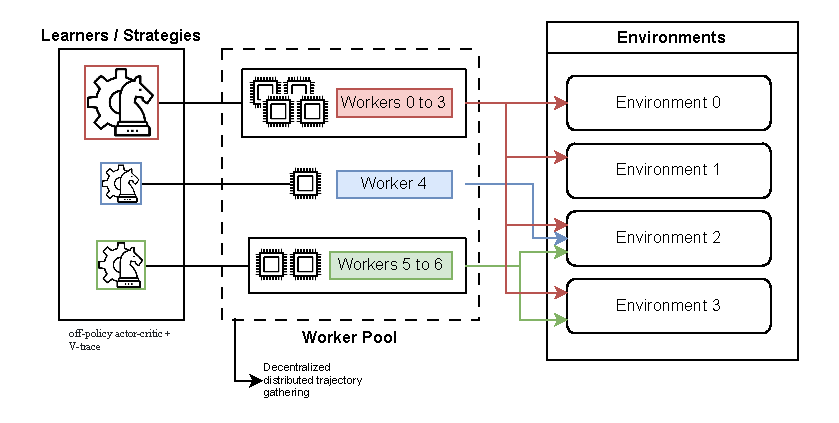
\includegraphics[width=\textwidth]{diagram}
    \caption{Diagram for the proposed parallel agent-based framework, with worker-learner interactions and shared limit order book environments.}
    \label{fig:framework}
\end{figure}

